\documentclass{article}

% Language setting
% Replace `english' with e.g. `spanish' to change the document language
\usepackage[T2A]{fontenc}
\usepackage[utf8]{inputenc}

% Set page size and margins
% Replace `letterpaper' with `a4paper' for UK/EU standard size
\usepackage[letterpaper,top=2cm,bottom=2cm,left=3cm,right=3cm,marginparwidth=1.75cm]{geometry}

% Useful packages
\usepackage{amsmath}
\usepackage{graphicx}
\usepackage{float}
\usepackage[colorlinks=true, allcolors=blue]{hyperref}
\usepackage{biblatex}
\usepackage{arabicore}

\title{Лабораторная работа №3}
\author{Выполнили: Цалов В.С. Тахватулин М.В.}

\begin{document}
\maketitle
\begin{center}
      {\fontsize{14}{15}\selectfont
            Преподователь: Оранский С.И.
      }
\end{center}
\section{Задание 1}
\subsection{Условие}
С помощью критерия согласия Пирсона хи-квадрат проверить согласованность
рейтинг футболиста с нормальным законом. Ту же самую задачу решить с помощью другого
критерия
\subsection{Выполнение}
Гипотезы: 
\begin{itemize}
      \item $H_0$: рейтинг футболистов распределен по нормальному закону
      \item $H_1$: рейтинг футболистов распределен по не норамльному закону
\end{itemize}
Алгоритм выполнения
\begin{enumerate}
      \item Суммируем рейтинг, чтобы получить величину
      \item Далее находим среднее и отклонение данной выборки
      \item Делаем выборку интервальной
      \item По найденым ранее параметра находим ожидаемые значения
      \item Находим $ \chi^2_{\text{набл}} $ и $ \chi^2_{\text{набл}} $
      \item Сравниваем их и определяем верную гипотезу
      \item Также проверяем гипотезы с помощью критерия Колмогорова-Смирнова
\end{enumerate}
\subsection{Код}
\subsection{Вывод программы}
Наблюдаемое значение хи-квадрат критерия: 11172.965189630037 \\ 
Критическое значение хи-квадрат критерия: 22.362032494826934 \\ 
Есть основания отвергать гипотезу $H_0$ $\rightarrow$ 1 гипотеза (ненормальное распределение) \\
Критерий Колмогорова-Смирнова:
Есть основания отвергать гипотезу $H_0$ $\rightarrow$ выборка распределена по не нормальному закону

\begin{figure}[H]
      \centering
      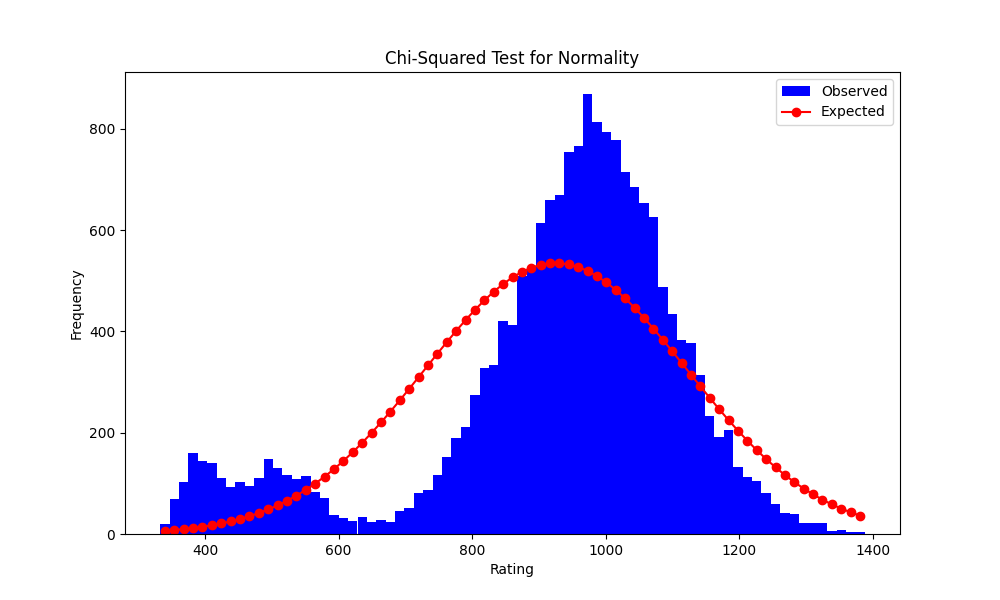
\includegraphics[width=1\linewidth]{../python/task1.png}
      \caption{Гистограмма распределения футболистов и ожидаемое нормальное распределение с полученными параметрами}\label{fig:figure}
\end{figure}
\subsection{Выводы}
Как критерий хи-квадрат, так и критерий Колмогорова-Смирнова опровергли гипотезу о том, что выборка рейтинга основана на нормальном законе. Также из графика видно, что это действительно так.

\section{Задание 2}
\subsection{Условие}
С помощью критерия однородности хи-квадрат проверить однородность рейтинга молодых и возрастных футболистов. Ту же самую задачу решить с помощью другого критерия
\subsection{Выполнение}
Гипотезы:
\begin{itemize}
      \item $H_0$: рейтинг молодых и возрастных футболистов однороден
      \item $H_1$: рейтинг молодых и возрастных футболистов не однороден 
\end{itemize}
Алгоритм выполнения:
\begin{enumerate}
      \item Делим футболистов по возрасту
      \item Разбиваем две выборки на интервалы
      \item После этого находим наблюдаемое и критическое значения
      \item Сравниваем их и опрделяем верную гепотезу
      \item Делаем тоже самое с помощью критерия Колмогорова-Смирнова
\end{enumerate}
\subsection{Код}
\subsection{Вывод программы}
Проверка гипотезы о том, что выборки молодых и возрастных футболистов однородны: \\
наблюдаемое значение критерия: 601.6660440175403 \\ 
критическое значение критерия: 4922.634987383697 \\ 
нет оснований отвергать нулевую гипотезу $ \rightarrow $ выборки однородны \\ 
Проверка гипотезы о том, что выборки молодых и возрастных футболистов однородны с помощью критерия Колмогорова-Смирнова: \\ 
Статистика Колмогорова-Смирнова: 0.12954988393062894 \\
p-значение: 1.364126296813217e-44 \\ 
Отвергаем нулевую гипотезу: выборки неоднородны.  \\
\begin{figure}[H]
      \centering
      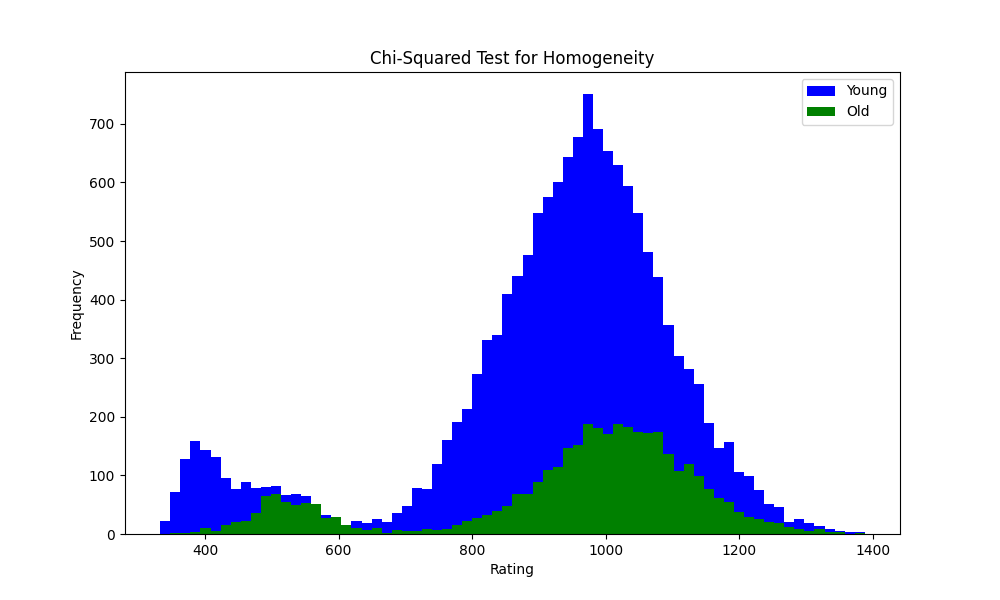
\includegraphics[width=1\linewidth]{../python/task2.png}
      \caption{Гистограмма распределения футболистов и ожидаемое нормальное распределение с полученными параметрами}\label{fig:figure}
\end{figure}
\subsection{Выводы}
Мы получили неоднозначный результат. Критерий хи-квадрать принимает гипотезу, а критерий Колмогорова-Смирнова отвергает.


\section{Задание 3}
\subsection{Условие}
С помощью критерия независимости хи-квадрат проверить независимость рейтинга и национальности футболиста. Ту же самую задачу решить с помощью другого критерия
\subsection{Выполнение}
Гипотезы:
\begin{itemize}
      \item $H_0$: Значения рейтинга зависят от национальности
      \item $H_1$: Значения рейтинга не зависят от национальности
\end{itemize}
Алгоритм выполнения:
\begin{enumerate}
      \item Составляем таблицу сопряженности
      \item Разбиваем колноку рейтинга на интервалы
      \item Находим наблюдаемое и критическое значение критерия
      \item Сравниваем и определяем гипотезу
\end{enumerate}
\subsection{Код}
\subsection{Вывод программы}
Наблюдаемое значение хи-квадрат критерия: 5002.698494943362
Критическое значение хи-квадрат критерия: 2499.7277366742187
Гипотеза $H_0$ отвергается $\rightarrow$ значения рейтинга не зависят от национальности
\end{document}